\section{CADO: Computer Aided Design Optimization Tool}
\todourgent[inline,author=Benni]{How did we put together the different parts? Here mainly first part of presentation: workflow, overview, user experience}
The absolute pipeline is illustrated in \autoref{fig:pipeline}
\begin{figure}[ht]
\begin{center}
		\begin{tikzpicture}[remember picture,auto,
    block/.style={
      rectangle,
      draw=blue,
      thick,
      fill=blue!20,
      text width=5em,
      align=center,
      rounded corners,
      minimum height=2em
    },
    block1/.style={
      rectangle,
      draw=blue,
      thick,
      fill=blue!20,
      text width=5em,
      align=center,
      rounded corners,
      minimum height=2em
    },
    line/.style={
      draw,thick,
      -latex',
      shorten >=2pt
    },
    cloud/.style={
      draw=red,
      thick,
      ellipse,
      fill=red!20,
      minimum height=1em
    }]
        \node [anchor=north,inner sep=0pt] [xshift=-4cm,yshift=0.7cm,inner sep=0pt](N1)
                {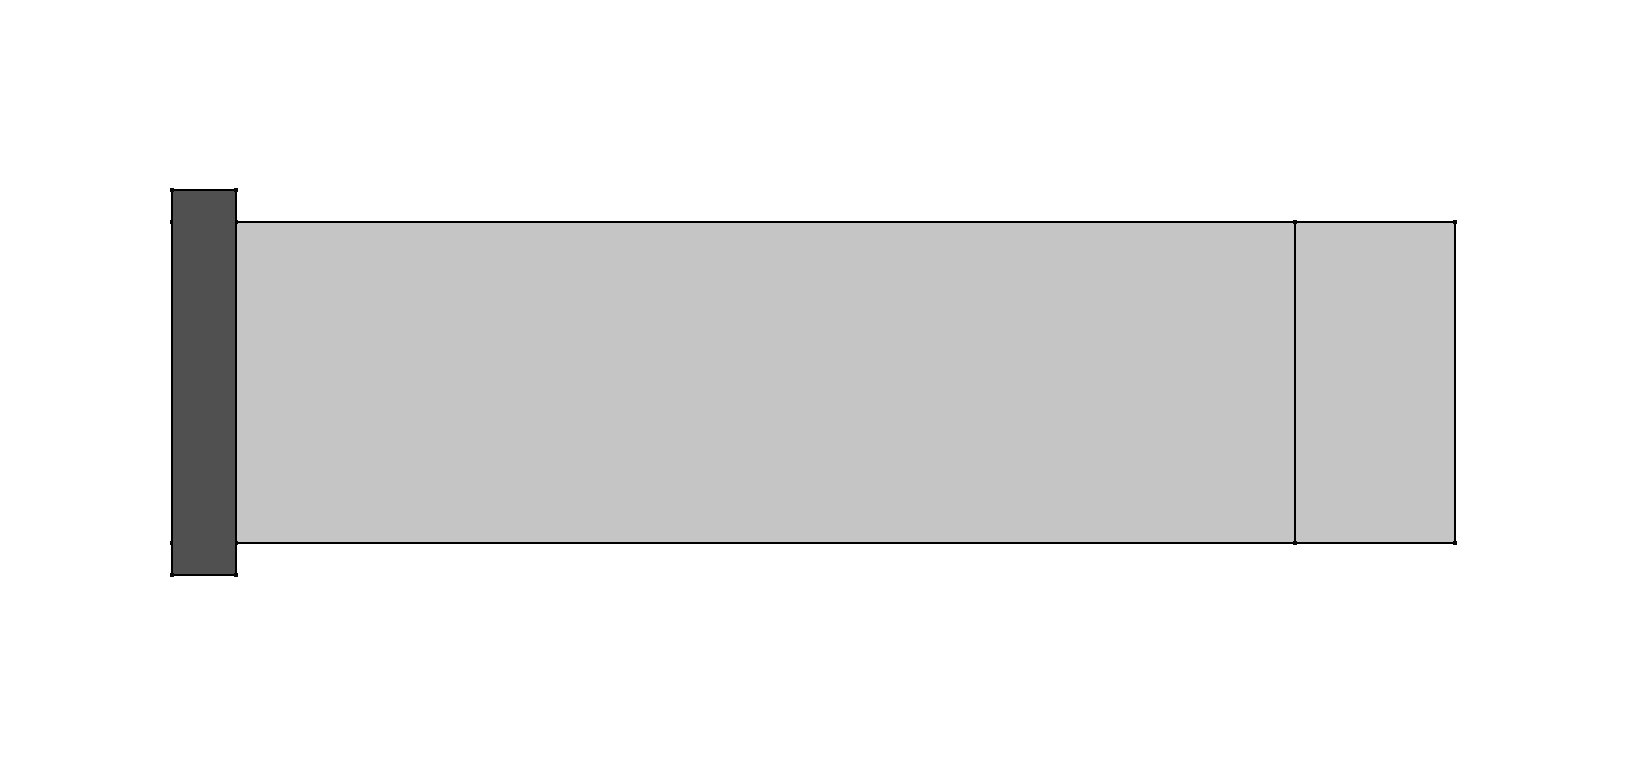
\includegraphics[scale=0.1]{Pictures/CADO_Overview/Back2CAD1.png}};
        \node [below =of N1,inner sep=0pt] [xshift=0cm,yshift=-0cm,inner sep=0pt](N5)
				{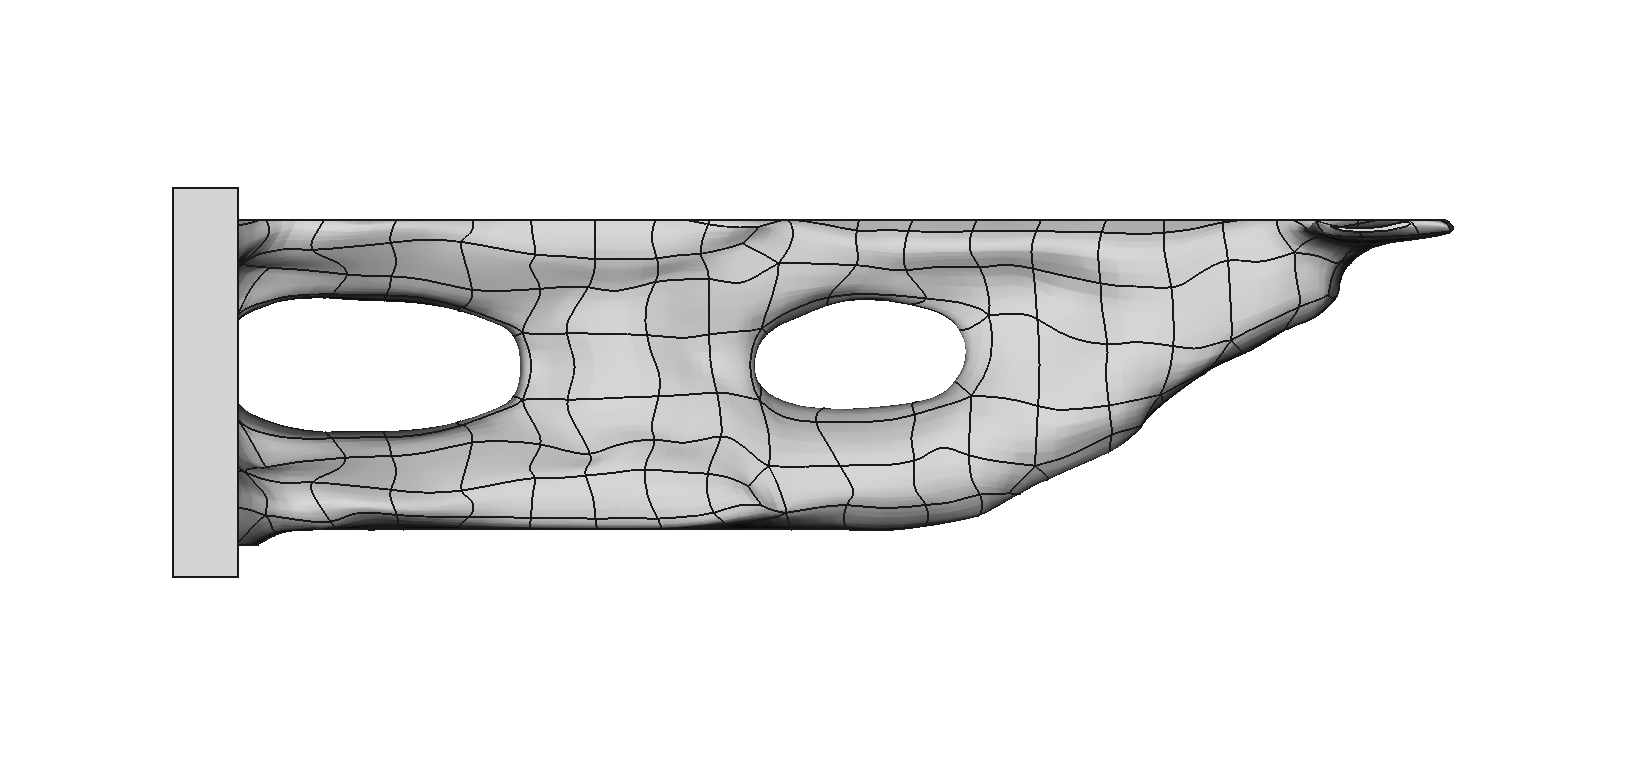
\includegraphics[scale=0.1]{Pictures/CADO_Overview/Back2CAD6.png}};
      	%\path[thick, ->,] (N5) edge [bend left] (N1); %node[yshift=-1.8cm, xshift = -0.1cm]{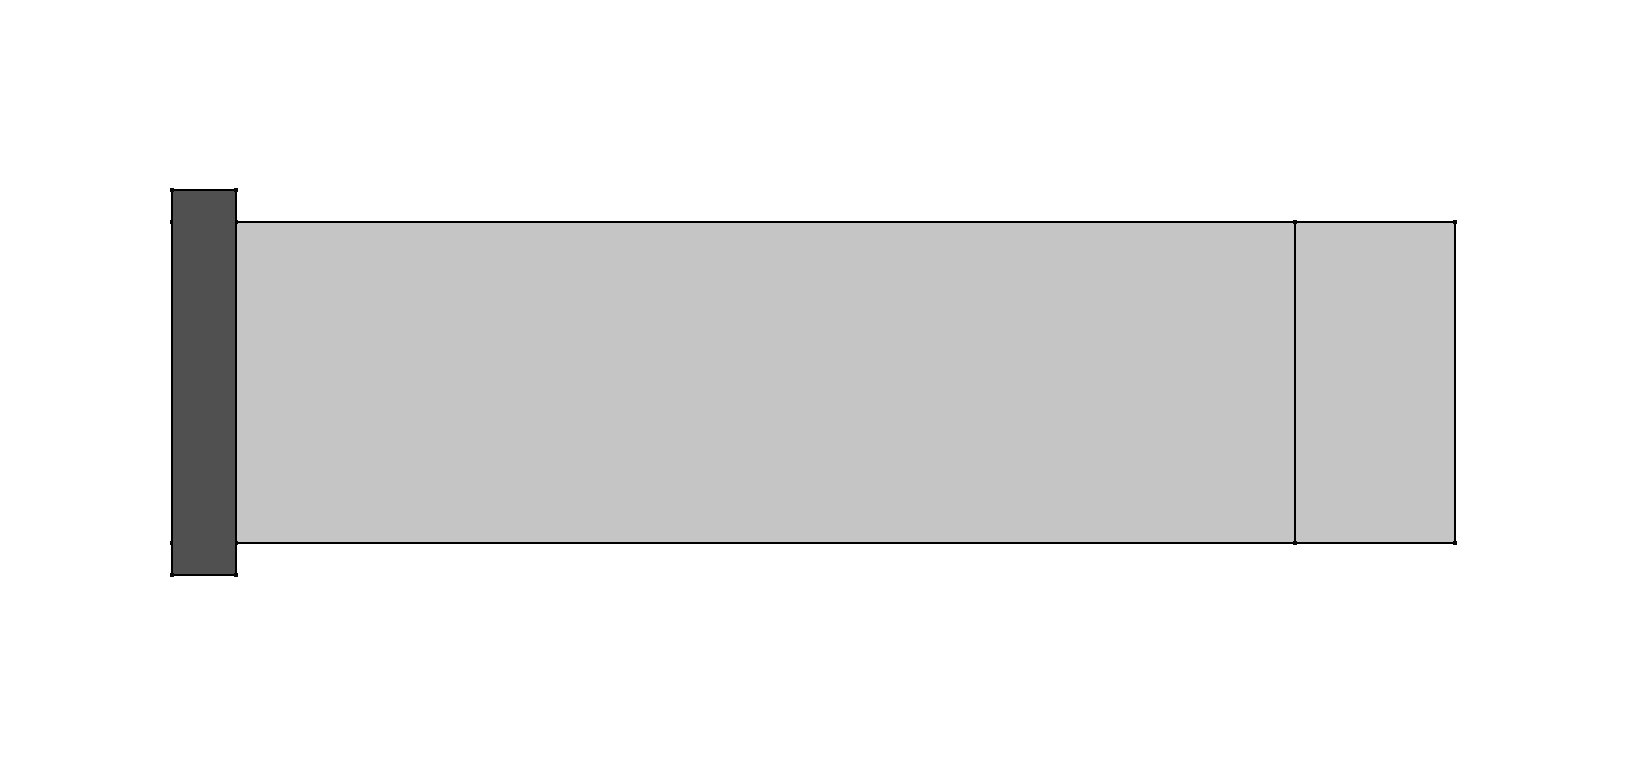
\includegraphics[scale=0.1]{Pictures/CADO_Overview/Back2CAD1.png}};
        \node [right =of N1,inner sep=0pt] [xshift=-1cm,yshift=3cm, inner sep=0pt](N2)             
                {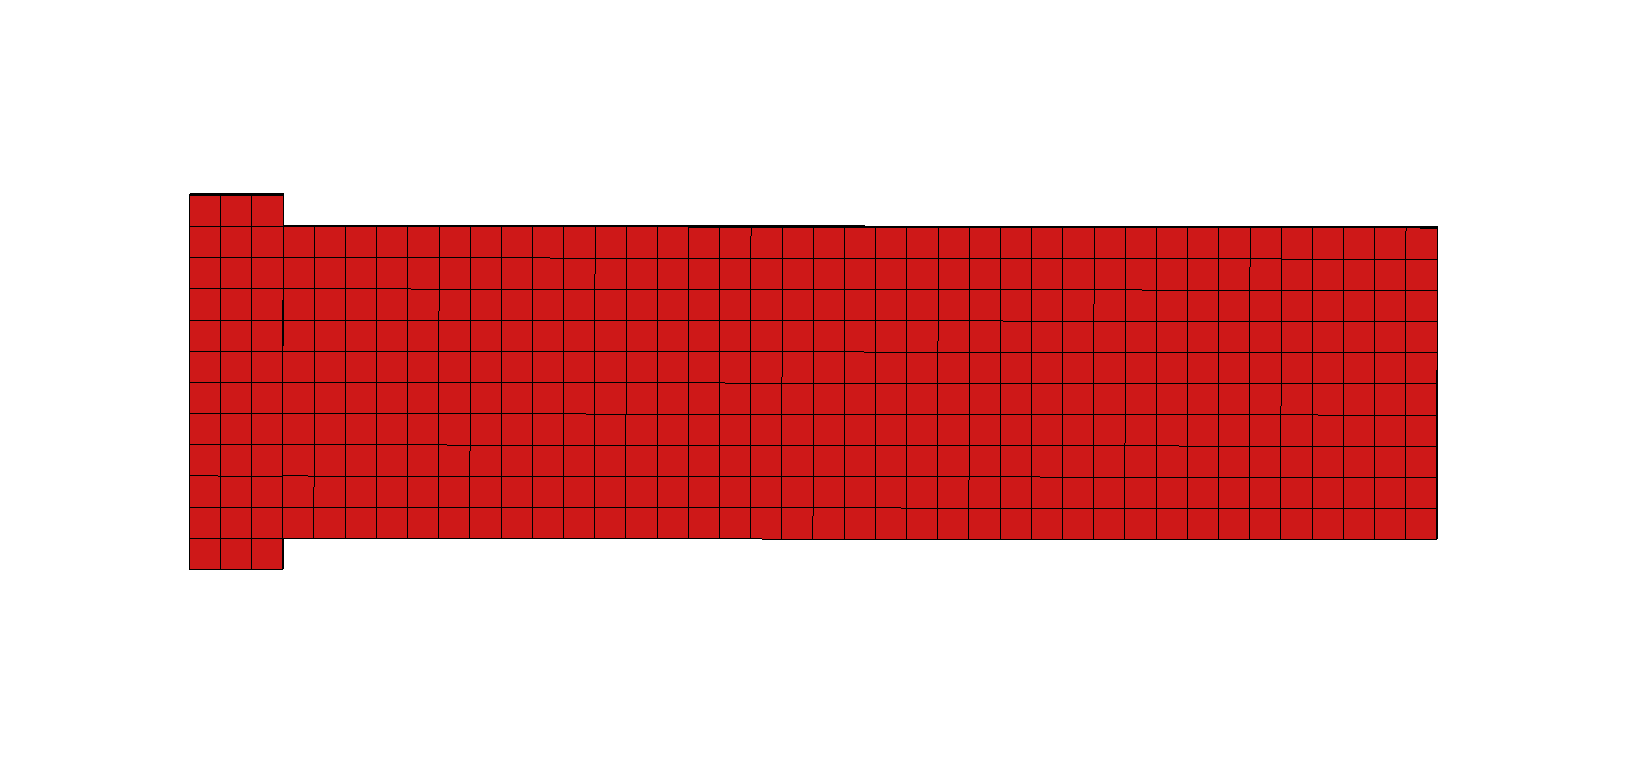
\includegraphics[scale=0.1]{Pictures/CADO_Overview/Back2CAD2.png}};
        \path[thick, ->] (N1) edge [bend left] (N2) node[yshift=0cm, xshift = -2.7cm]{(a)};
        \node [right =of N2,inner sep=0pt] [xshift=-1cm,yshift=-3cm, inner sep=0pt](N3) 
                {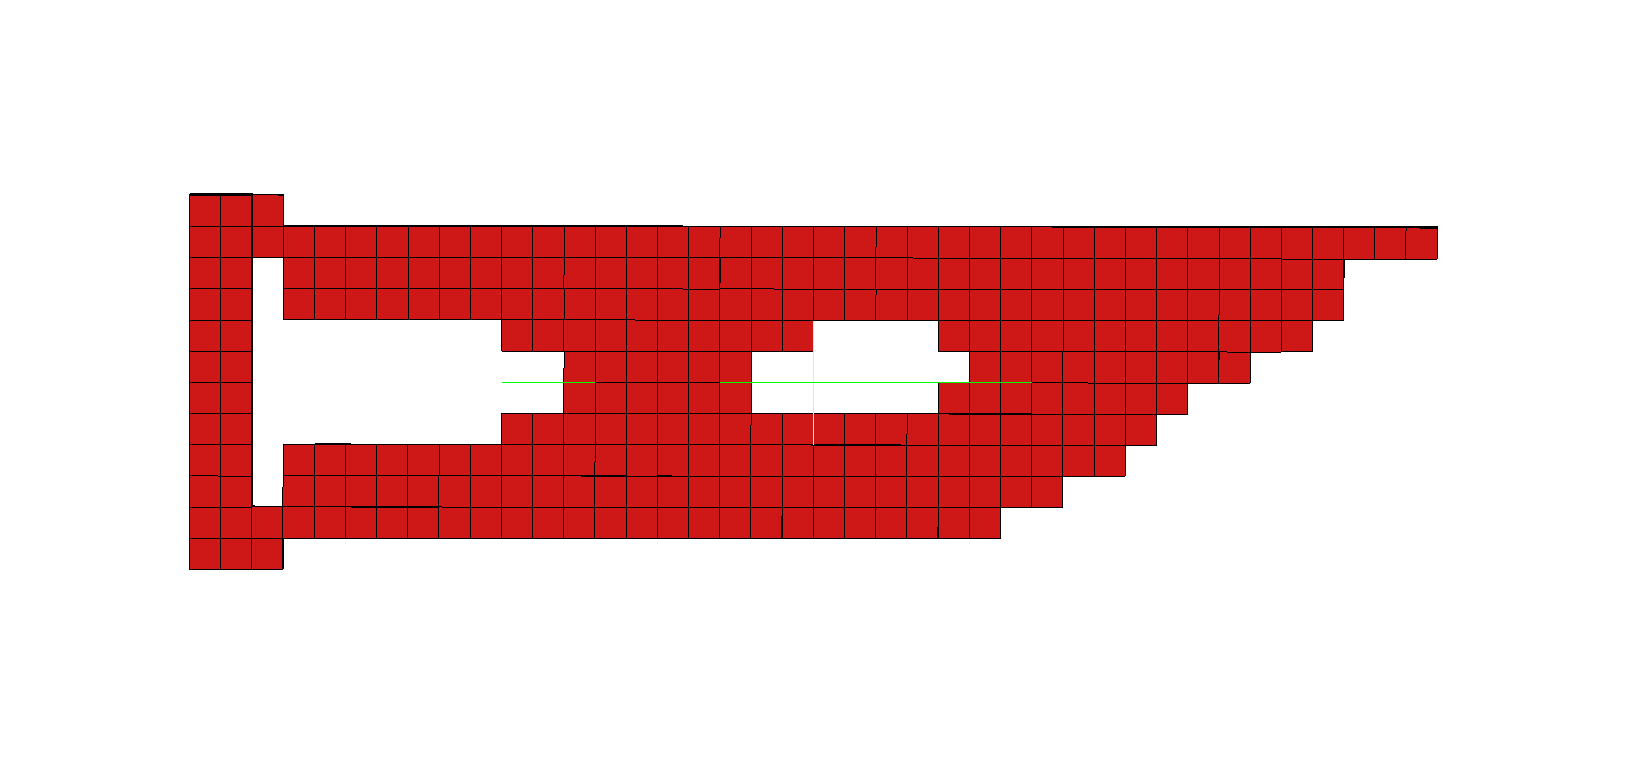
\includegraphics[scale=0.1]{Pictures/CADO_Overview/Back2CAD3.png}};
        \path[thick, ->] (N2) edge [bend left] (N3) node[yshift=1cm, xshift = 0.1cm]{(b)};
        \node [below =of N3,inner sep=0pt] [xshift=0cm,yshift=-0cm, inner sep=0pt](N4)
                {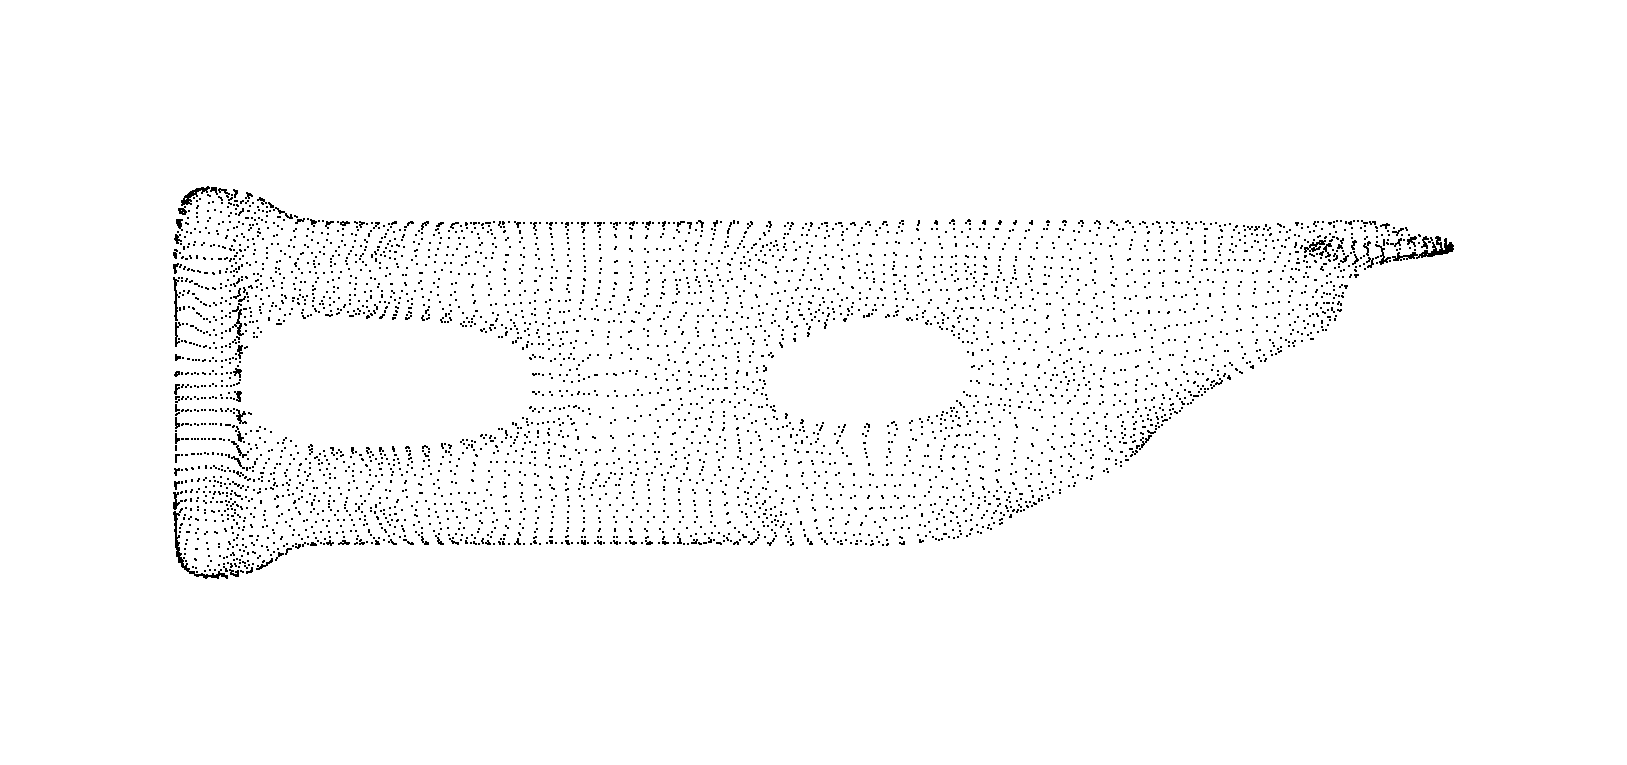
\includegraphics[scale=0.1]{Pictures/CADO_Overview/Back2CAD4.png}};
        \path[thick, ->] (N3) edge [bend left] (N4) node[yshift=0cm, xshift = 2.7cm]{(c)};
        \node [right =of N5,inner sep=0pt] [xshift=-0.7cm,yshift=-3cm, inner sep=0pt](N6)
                {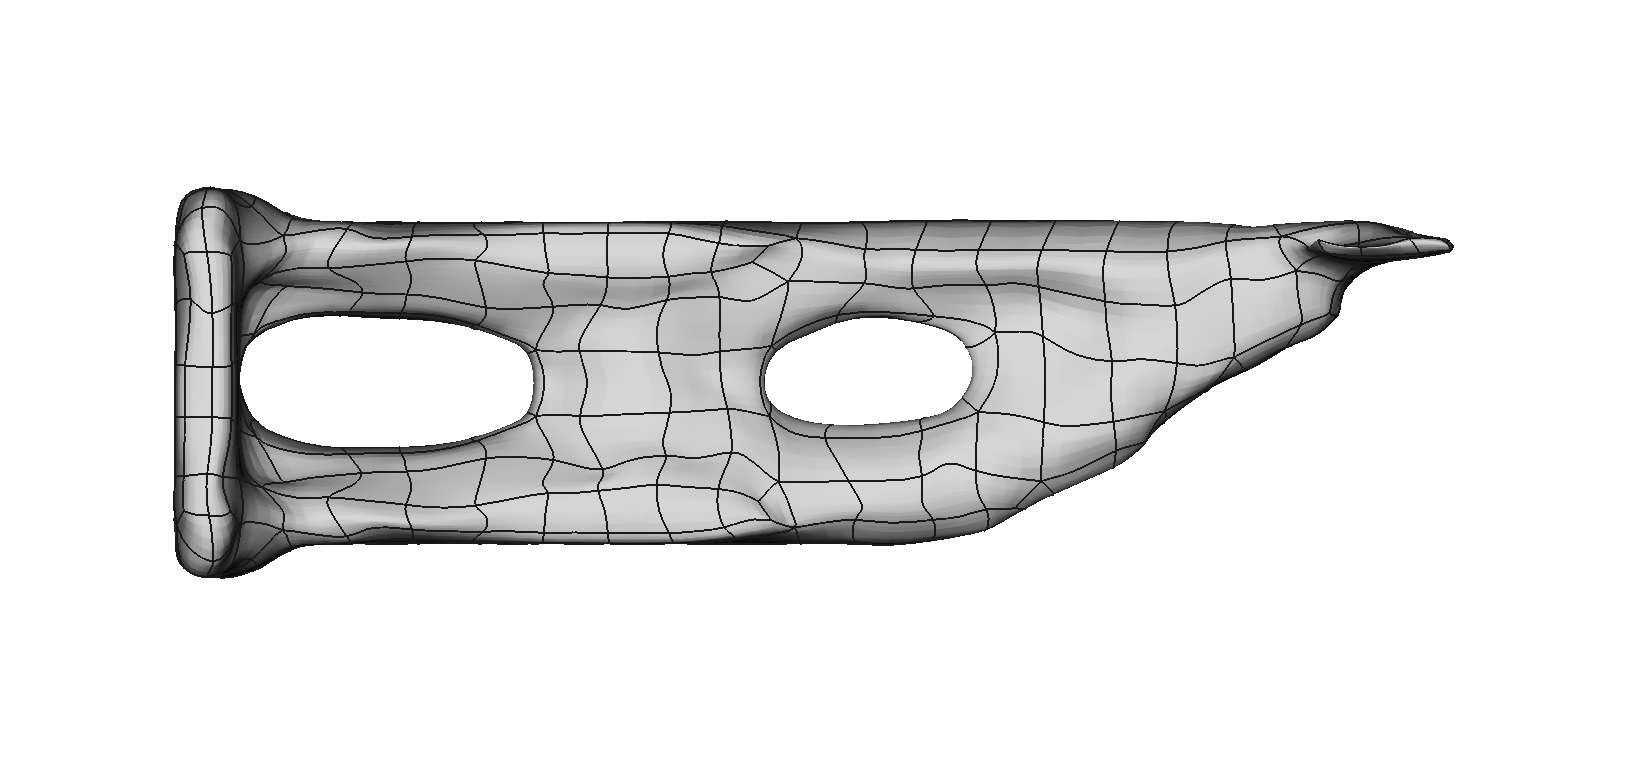
\includegraphics[scale=0.1]{Pictures/CADO_Overview/Back2CAD5.png}};
        \path[thick, ->] (N4) edge [bend left] (N6) node[yshift=0cm, xshift = 2.7cm]{(d)};
        \path[thick, ->] (N6) edge [bend left] (N5) node[yshift=-1cm, xshift = 0.1cm]{(e)} node[yshift=3cm, xshift = -8.7cm]{(f)};
        \end{tikzpicture}
        \caption{The workflow of CADO. From the given geometry (a) we start off by voxelizing (b). Next, topology optimization is applied (c) and the control points are computed (d). After computing the surface (e), finally, the boolean operation is executed and the final geometry is received (f).}
        \label{fig:pipeline}
	\end{center}
\end{figure}